\documentclass{article}[12pt]

\usepackage[english]{babel}
\usepackage[letterpaper,top=2cm,bottom=2cm,left=3cm,right=3cm,marginparwidth=1.75cm]{geometry}
\usepackage{amsmath}
\usepackage{graphicx}
\usepackage[colorlinks=true, allcolors=blue]{hyperref}

\title{Optimization and Scalability of Weightless Neural Networks: A Comprehensive Study}
\author{Artem Grigor, Georg Wiese}
\date{\today}

\begin{document}
\maketitle

\begin{abstract}
This report dives into the exploration and development of optimization techniques aimed at enhancing the performance and scalability of Weightless Neural Networks (WNNs).
Through a thorough investigation, various strategies including data preprocessing, feature extraction, and novel model construction methodologies have been proposed and evaluated.
The analyses and findings presented herein offer insight into the potential pathways toward achieving more efficient and scalable WNN architectures, opening up opportunities for their wider application in machine learning tasks.
\end{abstract}

\newpage
\tableofcontents
\newpage


\newpage
\section{Optimising the Prover}\label{sec:optimising-architecture}

The architecture of the Weightless Neural Networks (WNN) employed in the Rust Prover has been optimized to improve efficiency without sacrificing the security integrity of the system.
Several steps were considered in this optimization process, including altering the hash functions, removing redundant proofs, and applying lookup compression.
Below, we discuss each of considered steps in detail.

\newpage
\subsection{Exploring Alternate Hash Functions}\label{subsec:exploring-alternate-hash-functions}

Initially, the MishMash hashing algorithm was designed with a hash function derived from raising the input to the power of three within a small finite field, and subsequently truncating the result to the desired length.
This design was primarily chosen due to its ease of implementation and low computational cost.
However, it lacked in cryptographic strength and seemed suboptimal for circuit settings.
This section dives into the alternative hash function designs we considered.


\subsubsection{Requirements}\label{subsubsec:requirements}

The criteria outlined for our hash function were as follows:

\begin{itemize}
    \item High degree of randomness to ensure that similar inputs do not produce similar outputs.
    \item Computational efficiency.
    \item Straightforward verification.
\end{itemize}

The original MishMash hash function fulfilled the criteria of being quick and random.
Verification was also fairly simple, necessitating only a three-degree gate, apart from the smaller finite field constraints.

However, the objective was to find a hash function that is even simpler to verify, possesses greater randomness, and is thus more secure.

\subsubsection{Design}\label{subsubsec:design}

A simple multiplicative inverse was considered as an alternative hash function, as its verification was anticipated to be simple, requiring just a single multiplication gate.

The main concern revolved around the capability of the resulting hash function to sufficiently randomize the input bits.

\subsubsection{Evaluation}\label{subsubsec:evaluation}

Replacing the MishMash hash function with the multiplicative inverse, we evaluated its performance on Small, Medium, and Large MNIST datasets.

The evaluation revealed a minor performance reduction, but the inverse was found to be sufficiently random as a hash function.
However, the small reduction in gate count—from a three-degree to a two-degree gate—did not justify this alteration.

\subsubsection{Further Work}\label{subsubsec:further-work}

Aiming to further enhance the hash function's randomness, the next step involved removing the constraints for smaller finite field emulation by employing the inverse on the full field.
This adjustment was expected to eliminate another four gates, reducing the total gate count to two.

This venture encountered a technical barrier: the Cuda library, used for parallel computation, supported operations only up to 64-bit integers, whereas our task necessitated handling 256-bit integers.
Two potential solutions were identified:

\begin{itemize}
    \item Transitioning from Cuda to an alternative parallelization framework that supports 256-bit integers.
    \item Developing a custom wrapper for Cuda to enable operations on 256-bit integers.
\end{itemize}

Although both solutions were viable, they required a significant amount of effort.
We concluded that the expected benefits did not justify such an investment, particularly considering that hashing was responsible for a small portion of the total circuit size, limiting the scope for improvement.


\subsection{Eliminating Unnecessary Proof Verifications}\label{subsec:removing-redundant-proofs}

Within the existing framework, various layers of the WNN undergo proof verification.
However, it was observed that verifying proofs at certain layers does not enhance the security posture of the system.
A common trait among these layers is the execution of an easily invertible function \( f \) on an input value \( in \), resulting in an output \( out = f(in) \), with the original input \( in \) no longer being referenced in subsequent layers of the WNN.

The rationale behind the redundancy of proof verification in these layers can be better understood by considering two constraint systems: one with the \( out == f(in) \) check (System A), and one without it (System B). The goal is to demonstrate that these systems are equivalent concerning the set of accepted assignments to \( out \).
By \("\)equivalent,\("\) we imply that the set of accepted assignments to \( out \) remains consistent, irrespective of whether the \( out == f(in) \) check is performed.

Suppose an additional assignment \( out_x \) is accepted by System B but not by System A. Given the easily invertible nature of function \( f \), an \( in_x \) can be determined such that \( f(in_x) = out_x \).
Since all other checks in the systems remain unchanged, it follows that \( out_x \) is also an accepted assignment for System A, thereby affirming the equivalence of the two systems.

This equivalence stands valid only when no constraints are placed on the input value \( in \).
A typical scenario warranting input constraints occurs when the aim is to prove that a particular input \( in \) is identified as a Cat by the WNN model.

Nonetheless, there might be additional constraints on the input, necessitating proof verification for all function transitions.
For example, in a competition to find an input identified as a Cat by the WNN model, the initial participant commits to their input.
Once the competition concludes, they reveal the input, validate the WNN model's output, and ensure that the input hash matches the committed value.
In such instances, skipping the proof verification is infeasible.
Therefore, enabling this optimization should be user-configurable.

Applicable layers for this optimization include:
\begin{itemize}
    \item Thermometer Encoding layer
    \item Permutation layer
\end{itemize}

It's important to note that the entire WNN model, strictly speaking, is invertible due to the lack of cryptographically secure hash functions.
While inverting might be computationally intensive, it's not deemed a major concern within the context of the Rust Prover.

\subsection{Compressing Multiple Values into Native Field Elements}\label{subsec:encoding-values}

In the operational milieu of the Rust Prover, computations are conducted in a field nearing \(2^{256}\) in size, though the largest numbers used rarely exceed \(2^{13}\).
This significant magnitude disparity offers an optimization avenue, particularly concerning lookups and certain sequential operations.
Rather than allocating a single field element to represent a single bit or number, the approach of compressing multiple values into a single field element was adopted.
This method enables a more compact representation and efficient processing.

Consider, for instance, a situation where all filter inputs must be compressed into a single field element before executing a hash function.
Traditionally, this task would demand a bit decomposition and recomposition process, which, although standard, incurs additional computational overhead.
By initially encoding multiple values into a single field element, the necessity for bit decomposition and recomposition is obviated, thereby saving some constraints and time.

Although the impact of this optimization might seem minor when viewed in isolation, its utility is amplified when applied to lookups, a topic explored in the ensuing section.
Utilizing this condensed representation, the expansive nature of our operational field is leveraged to execute operations on encoded values more efficiently.
This not only boosts the performance of the Rust Prover but also potentially sets the stage for further optimizations in managing the WNN's constraint systems, as discussed in the section on eliminating unnecessary proof verifications in Section~\ref{sec:optimising-architecture}.



\subsection{Optimising Lookups}\label{subsec:lookups-optimisation}

Lookups account for a substantial portion of the constraints, approximately 70\%, making their optimization vital for enhancing the efficiency of the Rust Prover.

\subsubsection{Folding}\label{subsubsec:folding}

Utilising a folding scheme presents a viable strategy for optimising lookups.
Recent developments in folding schemes like \href{https://geometry.xyz/notebook/sangria-a-folding-scheme-for-plonk}{Sangria} now support the folding of custom PLONK gates, which can be utilized for implementing lookups.
Additionally, frameworks like \href{https://hackmd.io/@aardvark/rkHqa3NZ2}{Origami} provide a direct blueprint for implementing lookups in HALO2. Although these schemes haven't been extensively audited, their potential to considerably reduce constraints is promising.
Given that the WNN involves numerous repeated lookups and operations, such as each discriminator performs identical operations just with different inputs, the reduction in constraints could be significant.

However, to the best of our knowledge, Origami hasn't been implemented, and Sangria remains inaccessible for direct usage in the Halo2 library.
We are hopeful that this situation will improve in the near future.

\subsubsection{Compression}\label{subsubsec:compression}

\paragraph{Lasso}

A recent innovation, \href{https://eprint.iacr.org/2023/1216}{Lasso}, has illuminated the path for lookup optimizations.
Lasso requires payment only for the lookups actually performed, while the rest of the lookup table is accessed freely.
Given that in WNN, on average, only 2 to 6 values out of \(2^{13}\) are looked up, the reduction in constraints could be significant, potentially accelerating operations by a factor of 1000, depending on the intrinsic costs of the scheme.

However, Lasso, being newly introduced, is not yet compatible with the Halo2 library.

\paragraph{Custom Compression}

To refine the lookup process further, we endeavoured to develop an efficient protocol capable of provably decoding the $i^{th}$ bit of $n$ bits encoded in a single field element within finite field arithmetic.
This protocol leverages the unique characteristic of numbers within a finite field, where some have square roots while others do not, to facilitate the encoding of bits.

Our protocol aims to compact $n$ bits into a single field element and to provide a proof for the value of any given $i^{th}$ bit among the encoded $n$ bits, remarkably within a single constraint.
This scheme emerged from the need to compress binary lookup tables with sparse read access and accelerate bit decomposition, significantly reducing the row size of such tables by a factor of $n$ with only a single additional constraint per looked-up value, by compressing multiple consecutive evaluations into a single field value.

To our knowledge, this protocol is the first of its kind and is currently under review.

At the heart of the protocol is a pre-computation phase dedicated to constructing an encoding table.
Once created, this table serves as a universal asset, negating any further recalculations.
Post this pre-computation, the encoding of $n$ bits becomes a straightforward task, leveraging the table.
For instance, encoding bits `[1, 0, 1]` requires identifying a number $x$ that adheres to a set of conditions based on the square root property of $x$ or $x$ offset by specific values—a process significantly expedited by the precomputed encoding table.

The decoding operation of the $i^{th}$ bit involves examining specific sums involving the encoding field element $\text{enc_v}$ and $2 \times i$ to determine whether they are squares, which in turn reveals the bit value.
The proof of the bit value utilizes the verifiability of the square root property: by providing the square root of a particular expression, it becomes possible to corroborate the $i^{th}$ bit value with a singular constraint.
As a result, the full decoding of all $n$ bits demands merely $n$ constraints, making this protocol a practical extension to our Lookup Compression scheme.

Regarding computational complexity, the pre-processing stage crucial for constructing the encoding table bears a time complexity of \(O(4^n)\) and a space complexity of \(O(2^n)\).
However, the encoding and decoding processes are significantly less computationally intensive, rendering this scheme a plausible candidate for augmenting the efficiency of the lookup process in our architecture.
We further expect that more efficient algorithms for constructing the encoding table will be discovered in the future, thereby reducing the time and space complexities of the pre-processing stage.

\paragraph{Earlier Approach: 3-Level Array Lookup}
Before exploring our custom compression scheme, we utilized a 3-level array lookup mechanism to optimize extraction of bit compressed with other bits and stored within finite field elements.
Recognising that a single field element could encapsulate up to \( M \) bits of information, we aimed to encode multiple index bits into one field element initially using simple concatenation.

The procedure bundled \( n \) indices together, with \( n < M \).
During lookups, we first determined a compression index \( comp\_index = index_i / n \), signifying a compression of \( n \) bits.
The compression at this stage was a concatenation \( f_1..f_n \), resulting in a number between 0 and \( 2^n \).

To ascertain the value of the \( i \)-th bit stored in the compression, several strategies were explored:

\begin{enumerate}
    \item \textbf{Decomposition:}
    \begin{itemize}
        \item Formulate \( pre\_part + flag_i \cdot 2^i + post\_part = f_1..f_n \),
        \item Range check \( 0 \leq pre\_part < 2^i \),
        \item Range check \( 2^i < post\_part < 2^n \),
    \end{itemize}
    necessitating \( 2^n \) lookup rows with 2 columns.

    \item \textbf{Index Combination Lookup:}
    A lookup table encompassing all possible combinations between \( n \) bit values and a bit index was created, enabling the direct extraction of the \( i \)-th bit, requiring \( 2^{(n \cdot n)} \) lookup rows with 3 columns.

    \item \textbf{Chunk Decomposition:}
    This strategy converted the problem into selecting a correct chunk of \( k \) bits from \( n \) bits, with the potential for recursive application.
    \begin{itemize}
        \item Establish \( chunk_0 = acc_0 \),
        \item \( chunk_i + acc_{i-1} = acc_i \),
        \item \( select\_chunk_j = select\_chunk_{j-1} + chunk_j \cdot (j == select_i) \),
    \end{itemize}
    necessitating \( 2^{(n-k)} \) rows and approximately 7 columns.
\end{enumerate}

The original compression schema proposed and employed in the previous milestone was a hybrid of strategies 2 and 3.
An optimization equation has been devised to evaluate the optimal chunk sizes, their quantity, and the point at which an index lookup should be executed.

For instance, in the previous milestone, we used Chunk Decomposition with \( k = 3, \) and \( n = 5, \) followed by an Index Combination Lookup where \( n = 3, \).
This necessitated \( 2^9 + 2^2 \) rows.

However, this solution displayed scalability issues.
There existed a threshold beyond which compression yielded diminishing returns.
Eventually, the cumulative cost of index combination lookups and chunk decompositions would surpass the cost of straightforward lookups.

Although the exact figures were elusive and necessitated solving the optimization equation to ascertain optimal chunk sizes and their count, the emergence of a scheme capable of compressing \( n \) bits into a single field element without escalating overhead prompted us to set aside the optimization dilemma.
Instead, our focus shifted towards refining the newly proposed compression scheme, which offered a more promising avenue for enhancing lookup efficiency and scalability.

\newpage
\section{Optimising Preprocessing in WNN}\label{sec:optimising-preprocessing-in-wnn}

Data preprocessing and feature extraction are familiar steps in traditional machine learning, with a track record of boosting model performance in many experiments.
Yet, their effectiveness remains largely untested in the realm of Weightless Neural Networks (WNNs).
The assumption that standard preprocessing and feature extraction techniques would work equally well with binary data and models is quite looming, especially given that most of these techniques are tailored for operations with floating-point numbers.

In the sections that follow, we present methods aimed at enhancing the performance of the cutting-edge WNN model BTHWeN\@.

\subsection{Data preprocessing}\label{subsec:data-preprocessing}
\subsubsection*{Data Augmentation}
Data augmentation is our first tactic to combat overfitting and to better equip the model for generalization by enlarging the training dataset with minor variations in the data.
Two conventional methods were employed.

Initially, we applied random shifts to the images.
For each data point in the training set, two values were selected at random: a horizontal shift and a vertical shift, with negative values representing shifts to the left or downward, respectively.

\begin{figure}[h]
    \centering
    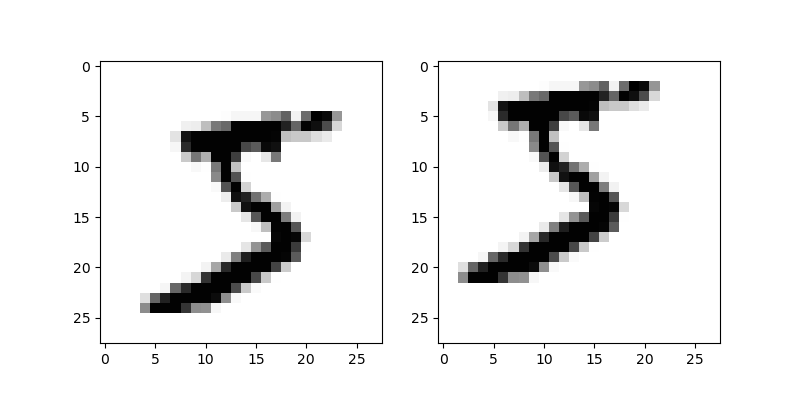
\includegraphics[width=0.5\textwidth]{imgs/img_shift}
    \caption{Data augmentation: image shifting}
    \label{fig:fig-1}
\end{figure}

A common approach in traditional machine learning is to add noise to the data, but this isn't a viable strategy for WNNs due to the necessity of binarizing the data.
Any noise added prior would be lost post-binarization, leading to identical binary data.
Hence, we suggest an alternative technique.

Post thermometer encoding, a specified number of bits are inverted.
Blindly inverting bits might yield unrealistic images and potentially hinder the model (e.g., altering central pixels inside the digit 0).
Therefore, we propose a defined method: initially, a probability \(p\) is set.
Following this, every black pixel with at least one white pixel neighbor can turn white with probability \(p\), and vice versa.
This process, while altering the image, retains its recognizability.
With the MNIST dataset, the numbers remain identifiable, albeit in varying handwriting styles (see~\ref{fig:fig-2}).

\begin{figure}[h]
    \centering
    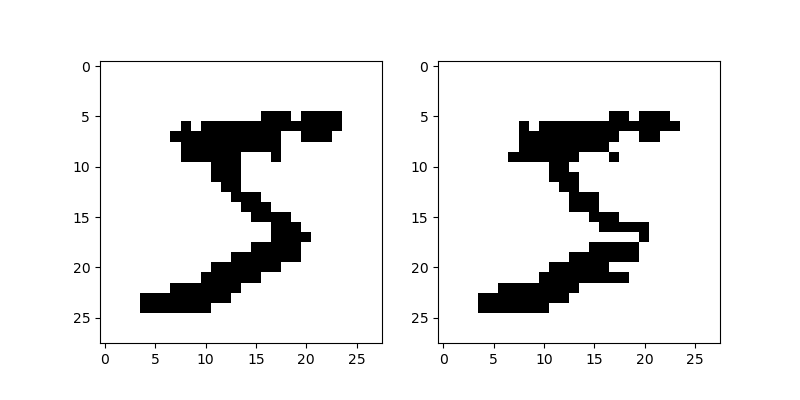
\includegraphics[width=0.5\textwidth]{imgs/img_corruption}
    \caption{Data augmentation: image corruption}
    \label{fig:fig-2}
\end{figure}

It's notable that data augmentation is particularly beneficial given the learning mechanism of WNNs, which essentially memorize each data point provided.
Hence, during inference, a slight shift in the image could stump the model.
A common workaround is to partition the image into pixel groups randomly, although this doesn't always yield the desired outcome as it heavily relies on the randomness of the partitioning.
Data augmentation can mitigate this randomness by diversifying the training data.

The data augmentation process doesn't impact the model's size or its processing speed during inference, although, as expected, it prolongs the training duration due to the enlarged dataset.

\subsubsection*{Discarding Non-informative Bits}
Post binarization, especially with thermometer encoding, certain non-informative bits emerge.
These bits are consistent (or nearly so) across all dataset observations (e.g., corner pixels being 0 for all images).
Evidently, such bits offer no insight regarding the class an observation belongs to.
We label these bits as \("\)bad\("\) and exclude them henceforth.
Therefore, when the image is divided into bit groups, these \("\)bad\("\) bits are left out.

\subsubsection*{Dimensionality Reduction}
In certain scenarios, there might be a need to reduce the data's dimensionality, for instance, when handling high-resolution images.
We are in pursuit of a relatively swift method that effectively shrinks the observation size.
Pooling (min, max, avg) emerges as such a method.
Given that the data is binarized anyway, employing this method doesn't entail a significant loss of information, provided the filter size is relatively small compared to the initial image.
Interestingly, some images might actually benefit from pooling, as it diminishes blurriness near color transition edges, which is favorable for binarization.

\subsection{Feature Extraction}\label{subsec:feature-extraction}

In any multilayer neural network, feature extraction is a fundamental capability, often harnessed in knowledge transfer.
We aimed to adopt the beneficial practices from traditional neural networks and adapt them for use in weightless neural networks (WNNs).
The goal was to enable the model to autonomously discern beneficial features from detrimental ones.
However, the challenge is, how can this be achieved without the luxury of classical model training?
Backpropagation, while a potent tool for conventional neural networks, renders models unexplainable.
Unlike most models, in WNNs, we can meticulously evaluate each learned feature and discard it if found to be redundant.

\subsubsection*{Feature Extraction Strategy}
Initially, it's crucial to understand what constitutes a feature in the context of a WNN\@.
While a single bit post-binarisation could technically be considered a feature, it often lacks substantial information on its own.
Henceforth, we'll define a feature as a cluster of bits routed to a specific filter.
In standard WNNs and BTHOWeN\footnote{The WNN structure in focus}, an observation is manually divided into bit groups, with each group assigned to a particular filter.
This setup allows us to identify which filter corresponds to which feature.
By assessing the performance of each filter independently, we can gauge the relevance of each feature.
The remaining task is to establish a measure of feature significance.

To address this, we need to clarify what we expect from an individual feature.
It's unreasonable to expect a single feature to accurately classify an observation.
A situation where a filter returns \textbf{1} only in the discriminator aligned with the class of the current observation is extremely unlikely, because a single feature could be common to multiple classes.
For instance, both digits \("6"\) and \("8"\) have a circular bottom, making \("\)having a circular bottom\("\) a useful feature as it helps the model instantly segregate these two digits from others using just this feature.
However, a feature like \("\)empty space in the image corner,\("\) despite returning \textbf{1} in the correct class discriminator, would also return \textbf{1} in all other discriminators, rendering it ineffective.
In essence, we want a filter representing a feature to consistently return \textbf{true} for its class, while returning \textbf{false} for at least some other classes.

To rigorously determine feature significance, we introduce two metrics.
Let's denote the set of features as $\mathcal{F} = \{f_k|k=1,\dots,M\}$ and each filter within a model as $\phi_{j,f_k}$, where $j$ is the number of discriminators (or number of classes) and $f_k$ is the feature corresponding to the given filter.
We define the accuracy of a feature as the ratio of occurrences when the filter associated with the feature in question returned \textbf{1} in the discriminator corresponding to the class of the considered observation (\ref{eq:acc-f}) to the total number of observations.
\begin{equation}\label{eq:acc-f}
    acc(f_k) = \frac{\sum_{i=1}^{N}\mathbf{1}_{\phi_{y_i,f_k}(x_i) = 1}(x_i)}{N}
\end{equation}
where $X = \{x_i|i=1,\dots,N\}, Y = \{y_i,i=1,\dots,N\}$ represent observations and labels respectively.
Next, we define the commonality of a feature as the ratio of discriminators for which the corresponding filter returned \textbf{1} to the total number of discriminators (number of classes) (\ref{eq:uni-f}), averaged over all observations.
A value of $ord(f_k) \approx 1$ indicates a feature akin to \("\)empty space in the image corner\("\) described earlier.
\begin{equation}\label{eq:uni-f}
    ord(f_k) = \frac{1}{N}\sum_{i=1}^{N}\frac{\sum_{j=1}^{C}\mathbf{1}_{\phi_{j,f_k}(x_i) = 1}(x_i)}{C}
\end{equation}
where $C$ denotes the number of discriminators (number of classes).

Subsequently, we introduce two hyperparameters $\alpha \in [0,1], \beta \in [0,1]$.
A feature is deemed $\alpha,\beta$-significant if:
\begin{equation}
    (acc(f_k) \ge \alpha) \wedge (ord(f_k) \le \beta)\label{eq:equation}
\end{equation}
and the set of $\alpha\beta$-significant features is represented as $\mathcal{F}^{\alpha\beta} = \{f_k| (acc(f_k) \ge \alpha) \wedge (ord(f_k) \le \beta)\}$.
Suitable values for $\alpha, \beta$ can be determined either through logical deduction (given their intuitive interpretation) or via a validation set.

With $\alpha\beta$-significance defined, we can now utilize this criterion for feature selection.
We suggest two applications for feature selection in WNNs: model reduction and model construction.

\subsubsection*{Model Reduction via Feature Selection}
Model reduction, based on $\alpha\beta$-significance, entails the removal of filters associated with $\alpha\beta$-insignificant features.
This method allows for model size reduction by discarding less important features.

\subsubsection*{Model Construction using a Greedy Algorithm for Feature Selection}
Typically, features for the BTHOWeN model (or other WNNs) are chosen through a random split of the binarised image into pixel groups.
This random approach doesn't ensure the inclusion of all useful features.
To build a model comprising important features, we propose the following greedy algorithm:
\begin{enumerate}
    \item
            Initialize $\mathcal{F}^{\alpha\beta} = \{\}$.
            Define hyperparameters $\alpha, \beta$ and the number of $\alpha\beta$-significant features to be included, denoted as $\gamma$.
    \item Generate $\mathcal{F}$ by randomly splitting the binarised image into pixel groups.
    \item For each $f_k$ in $\mathcal{F}$:
    \begin{enumerate}
        \item Train a model with a single feature.
        \item On the validation set, find the bleach value that ensures $ord(f_k) \le \beta$ while maximizing $acc(f_k)$.
        \item If $acc_{\max}(f_k) \ge \alpha$ and $f_k$ doesn't share more than half of its pixels with any $f^{\alpha\beta} \in \mathcal{F}^{\alpha\beta}$ (to avoid similar features), add $f_k$ to set $\mathcal{F}^{\alpha\beta}$ and save its optimal bleach value.
        \item If $|\mathcal{F}^{\alpha\beta}| = \gamma$, halt the process.
    \end{enumerate}
    \item If $|\mathcal{F}^{\alpha\beta}| < \gamma$, revert to step 2.
\end{enumerate}
Note, this algorithm not only facilitates the creation of a set of $\alpha\beta$-significant features but also approximates the best bleaching value for each feature, enabling the model to learn more sophisticated patterns.

\subsection{Evaluation of Data Preprocessing and Feature Selection}\label{subsec:evaluation-of-data-preprocessing-and-feature-selection}

The methods of data preprocessing and feature selection laid out earlier can be utilized in various combinations.
The suitability and effectiveness of each method should be gauged individually for each task.
Additionally, the success of a preprocessing method is also influenced by the model architecture.
Below are some conclusions drawn from simulations:

\subsubsection{Outcomes on Data Augmentation}
Data augmentation can enhance the model's performance, but necessitates a larger WNN model since WNN learns by recognizing certain patterns.
Data augmentation creates data with a wider variety of patterns.
Hence, a larger model is needed to identify all possible patterns, otherwise, we encounter an issue where the hashing function begins to map different patterns to identical values.
Thus, when employing data augmentation with small models, practitioners should exercise caution as it might degrade the performance (see table~\ref{tab:table-1}).
\begin{table}[h]
    \centering
    \begin{tabular}{|c|c|}
    \hline
    model & accuracy \\
    \hline
       Small MNIST &  0.924\\
    \hline
       Small MNIST with data augmentation  & 0.913\\
    \hline
       Large MNIST &  0.945\\
    \hline
       Large MNIST with data augmentation  & 0.948\\
    \hline
    \end{tabular}
    \caption{Comparing models on MNIST dataset with and without data augmentation. Small model specifications: bits per input = 2, unit inputs = 28, unit entries = 1024, unit hashes = 2, Large model specifications: bits per input = 6, unit inputs = 49, unit entries = 8192, unit hashes = 4}
    \label{tab:table-1}
\end{table}

For smaller models, applying pooling may be beneficial.
As mentioned earlier, small models struggle to learn a variety of different patterns.
Pooling reduces the size of the observations while preserving important patterns (see table~\ref{tab:table-2}).
Note, for the same models, the model applied to data with pooling with window $2\times{}2$ has half the filters, thus is half the size.
As a result, we have a model that is half as small, but its accuracy is only 1\% lower.
\begin{table}[h]
    \centering
    \begin{tabular}{|c|c|}
    \hline
    model & accuracy \\
    \hline
       Tiny MNIST &  0.887\\
    \hline
       Tiny MNIST, max pooling with window 2 by 2  & .876\\
    \hline
    \end{tabular}
    \caption{Tiny model on MNIST dataset with and without pooling. Tiny model specifications: bits per input = 2, unit inputs = 9, unit entries = 128, unit hashes = 1}
    \label{tab:table-2}
\end{table}

\subsubsection{Outcomes on Model Reduction using Feature Selection}
The experiments conducted reveal that the proposed method enables effective model size reduction by removing filters linked to $\alpha\beta$-insignificant features.
The table shows that even for a small model, we were able to cut the model size by half (removing 24 features out of 56), with only a 1.3 percent drop in accuracy.
\begin{table}[h]
    \centering
    \begin{tabular}{|c|c|}
    \hline
    model & accuracy \\
    \hline
       Small MNIST &  0.924\\
    \hline
       Small MNIST with feature selection  & 0.911\\
    \hline
    \end{tabular}
    \caption{Small model on MNIST dataset with and without features selection. Small model specifications: bits per input = 2, unit inputs = 28, unit entries = 1024, unit hashes = 2}
    \label{tab:table-22}
\end{table}

\subsubsection{Outcomes on Model Construction using Feature Selection}
The greedy algorithm detailed earlier is computationally demanding, which notably extends the model's training time.
Based on the experiments, it is concluded that for simpler datasets, applying this algorithm isn't reasonable in most cases if model parameters are properly adjusted, as it offers minimal accuracy improvement.
For instance, on the MNIST dataset, if we set \texttt{unit\_entries}\footnote{hyperparameters names are carried over from the article where the BTHOWeN model is introduced} greater than 28 (number of bits counted as one feature), the likelihood of any feature being insignificant is very low.
Consequently, the model built by the proposed greedy algorithm exhibits nearly the same performance (see table).
Nonetheless, for larger and more complex datasets, this method is anticipated to yield better results.

\subsubsection{Merging Approaches} \label{subsubsec:best-res}
For attaining a model with superior performance, a blend of the proposed methods can be employed.
The procedure that aided in achieving a better model on the MNIST dataset, compared to the BTHOWeN model of a similar size, is described below:

\begin{enumerate}
    \item Apply max pooling to the images with a kernel of size $2\times{}2$.
    \item Apply thermometer encoding with bits per input = 2
    \item Identify uninformative bits and label them as \("\)bad\("\)
    \item Generate features.
          Rather than creating random features, a sliding window of size $3 \times 3$ is defined and placed in each possible position.
          If no bit is \("\)bad\("\), this combination of bits is added to features.
    \item Following this procedure, numerous features are obtained, many of which overlap with each other.
          Therefore, a model is constructed using the greedy algorithm for feature selection.
\end{enumerate}

For this method, the following parameters for the model were defined: bits per input = 2, unit inputs = 9, unit entries = 512, unit hashes = 2.
The number of features used is 125\footnote{Note that if data preprocessing and feature selection weren't applied, the total number of features for 2 bits per input would be $(28-3+1)^2 = 676$}.
Thus, a model of roughly the same size as the MNIST small model from the article \cite{susskind2022weightless} (MNIST small model has double the filter size, but our model has double the filters) was obtained, but with 1\% better accuracy.
The accuracy for the given model is equal to 0.944.


\section{Scaling WNN}\label{sec:scaling-wnn}
Training WNNs for more complex datasets having many features inevitably leads to a significant increase in the model size and, consequently, inference time \cite{aleksander2009brief}.
To address this issue, we can employ certain techniques mentioned earlier.

Firstly, we can apply pooling, which significantly reduces the size of the data.
However, it's important to note that some information may be lost due to this operation.

Secondly, we can remove uninformative bits.
This operation doesn't eliminate any information, but it's worth noting that not every dataset contains such bits.

Thirdly, we can utilize the feature selection algorithm proposed earlier.
Instead of using all the bits from the encoded observations, we can explicitly control the number of features we want to use and sample significant features using the proposed greedy algorithm.
As demonstrated in section~\ref{subsubsec:best-res}, this combination of methods can dramatically reduce the model's size and, with careful hyperparameter tuning, even improve accuracy.

As an illustrative example, we attempted to fit the BTHOWeN model to the CIFAR-10 dataset.
Even the Large MNIST model from the article~\cite{susskind2022weightless} resulted in an accuracy of only 0.43.
This suggests that it may be necessary to significantly increase the size of the model, apply the aforementioned approaches, or a combination of both, to achieve satisfactory performance.

\section{Translating DNN into WNN}\label{sec:translating-dnn-into-wnn}
Translating DNNs into WWNs is a challenging task.
Binarizing the weights is not a viable option, as rounding weights to 0 or 1 for a trained DNN effectively results in a completely new DNN\@.
Theoretically, one approach is to extract features from a DNN, which can then be used for feature selection in a WNN\@.
However, this approach immediately encounters the unsolved problem of creating an interpretable deep neural network.

Some attempts have been made to create interpretable neural networks by combining Formal Concept Analysis with neural networks~\cite{parakal2022intrinsically, dudyrev2022human, kuznetsov2022pattern}.
However, this represents a relatively new direction in neural network research, and as of now, there are no universally satisfying results in this area.

\section{Efficiently Training WNN}\label{sec:training-wnn}
Traditional training methods for WNNs are not applicable, as gradient descent works only with floating-point numbers and cannot be directly applied to discrete tasks.
In light of this, we can only propose a high-level concept, which is still in its early stages of exploration.

Firstly, we may attempt to formulate the task of training the WNN model as a discrete optimization problem.

Secondly, many discrete optimization tasks can be reduced to a Quadratic Unconstrained Binary Optimization (QUBO) problem, which involves minimizing a second-degree polynomial where all variables are either 0 or 1.
This problem is equivalent to finding the ground state in the Ising model, where the corresponding spin variables are either -1 or 1.
Essentially, we need to find a spin configuration that minimizes the Hamiltonian of the Ising model~\cite{glover2018logical}.
This problem can further be reduced to solving a system of differential equations \cite{goto2019combinatorial, goto2021high}.

Hence, we may explore the possibility of constructing a transition from a discrete (binary) problem to a continuous problem and then investigate how classical training algorithms can be adapted for use in this context.


\newpage
\bibliographystyle{abbrv}
\bibliography{sample}

\end{document}